\documentclass{beamer}
\usetheme{Boadilla}

\usepackage{amsmath}
\usepackage{amsfonts}
\usepackage{hyperref}

\usepackage{amsmath}
\DeclareMathOperator*{\argmax}{arg\,max}
\DeclareMathOperator*{\argmin}{arg\,min}

\title{BMA under Covariate Shift}
\author{Timofey Chernikov}
\institute{MIPT, 2023}


\begin{document}

\begin{frame}
    \titlepage
\end{frame}


% \begin{frame}
%     \tableofcontents
% \end{frame}


\section{Introduction}
\begin{frame}{Introduction}
    \begin{block}{Main idea}
        Bayesian neural networks (BNNs) with high-fidelity approximate
        inference via full-batch Hamiltonian Monte Carlo achieve poor generalization
        under covariate shift, even underperforming classical estimation.
        We explain this surprising result. We additionally show why the same
        issue does not affect many approximate inference procedures, or classical maxi-
        mum a-posteriori (MAP) training. Finally, we propose novel priors that improve
        the robustness of BNNs to many sources of covariate shift.
    \end{block} 
\end{frame}

\begin{frame}{Introduction}
    \begin{block}{Bayesian neural networks}
        A Bayesian neural network model is specified by the prior distribution
        $p(w)$ over the weights $w$ of the model, and the likelihood function $p(y|x, w)$, where $x$ represents the
        input features and $y$ represents the target value.

        Following Bayes’ rule, the posterior distribution over the parameters w is given by

        $$ p(w|D) = \frac {p(D|w)p(w)} {\int p(D|w')p(w')dw'} $$

        $$ p(y|x) = \int p(y|x,w)p(w|D)dw $$
    \end{block} 
\end{frame}

\begin{frame}{Introduction}
    \begin{block}{Maximum a-posteriori (MAP) estimation}
        In contrast with Bayesian model averaging, a MAP
        estimator uses the single setting of weights (hypothesis) that maximizes the posterior density
        $w_{MAP} = argmax p(w|D) = argmax(log p(D|w) + log p(w))$, where the log prior can be viewed
        as a regularizer. In other words, the MAP estimator is a classical neural network approach.
    \end{block}
    
    \begin{block}{Covariate shift.}
        In this paper, we focus on the covariate shift setting. We assume the training
        dataset $D_{train}$ consists of i.i.d. samples from the distribution $p_{train} (x, y) = p_{train} (x) · p(y|x)$. 
        However, the test data may come from a different distribution 
        $p_{test} (x, y) = p_{test} (x) · p(y|x)$. For concreteness,
        we assume the conditional distribution $p(y|x)$ remains unchanged, 
        but the marginal distribution of the input features $p_{test} (x)$ differs from $p_{train} (x)$.
    \end{block}
\end{frame}


\section{Comparison}
\begin{frame}{Comparison}
 \begin{block}{Methods}
    We evaluate BNNs against two deterministic baselines: a MAP solution approximated
    with stochastic gradient descent (SGD) with momentum and a deep ensemble of 10 independently 
    trained MAP solutions. For BNNs, we provide the results using a Gaussian prior and a
    more heavy-tailed Laplace prior. Izmailov et al. conjectured that
    cold posteriors can improve the robustness of BNNs under covariate shift; to test this hypothesis,
    we provide results for BNNs with a Gaussian prior and cold posteriors at temperature $10^{-2}$. For all
    BNN models, we run a single chain of HMC for 100 iterations discarding the first 10 iterations as
    burn-in, following Izmailov et al. We provide additional experimental details in Appendix A.
    \end{block}
\end{frame}

\begin{frame}{Methods}
\begin{block}{Neural network architectures}
    On both the CIFAR-10 and MNIST datasets we use a small
    convolutional network (CNN) inspired by LeNet-5, with 2 convolutional layers followed by
    3 fully-connected layers. On MNIST we additionally consider a fully-connected neural network
    (MLP) with 2 hidden layers of 256 neurons each. We note that high-fidelity posterior sampling with
    HMC is extremely computationally intensive. Even on the small architectures that we consider, the
    experiments take multiple hours on 8 NVIDIA Tesla V-100 GPUs or 8-core TPU-V3 devices.
    \end{block}
\end{frame}

 

\section{Model}
\begin{frame}{}
\begin{block}{Test data corruption}
    We start by considering the scenario where the test data is corrupted by some type of noise. In this
    case, there is no semantic distribution shift: the test data is collected in the same way as the train data,
    but then corrupted by a generic transformation.
\end{block}
    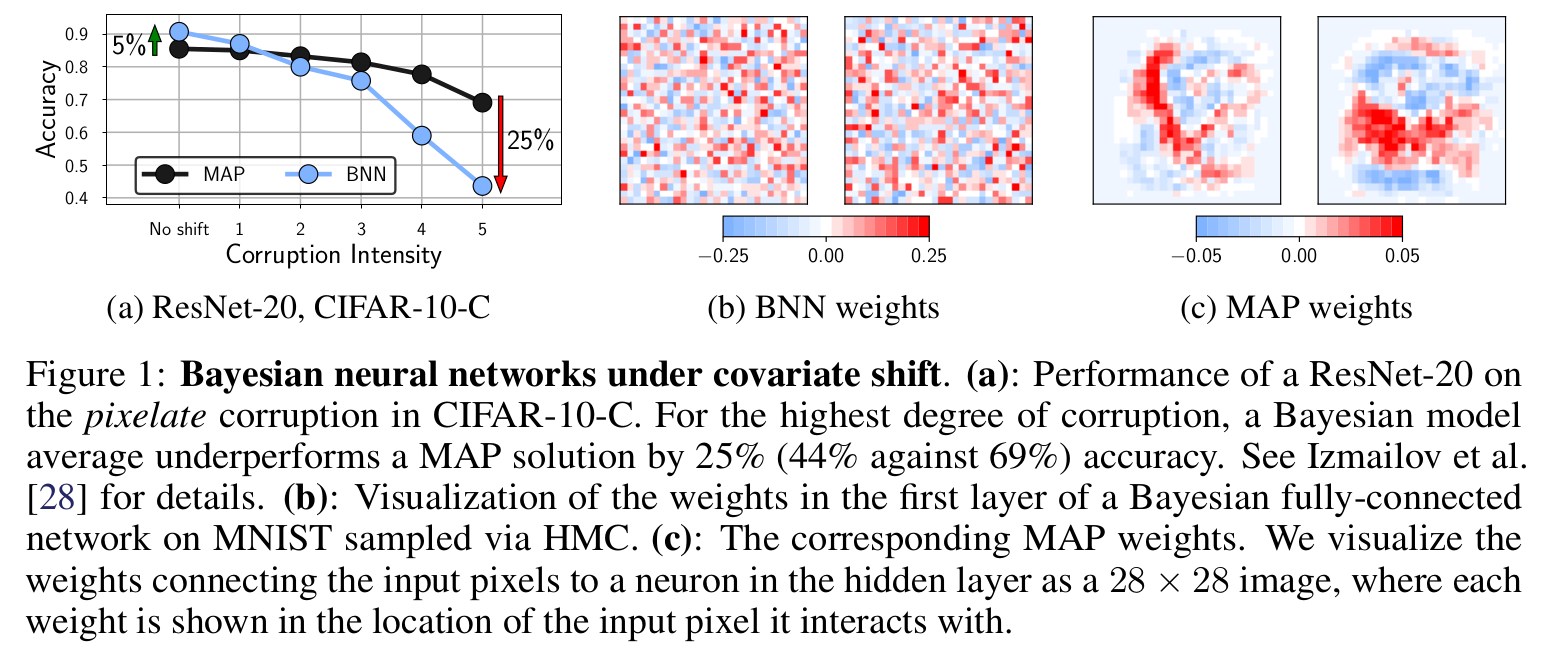
\includegraphics[scale=0.22]{figure1.png}
\end{frame}

\begin{frame}{}
\begin{block}{Domain shift}
    Next, we consider a different type of covariate shift where the test data and train data come from
    different, but semantically related distributions.
    First, we apply our CNN and MLP MNIST models to the SVHN test set. The MNIST-to-
    SVHN domain shift task is a common benchmark for unsupervised domain adaptation.
\end{block}
    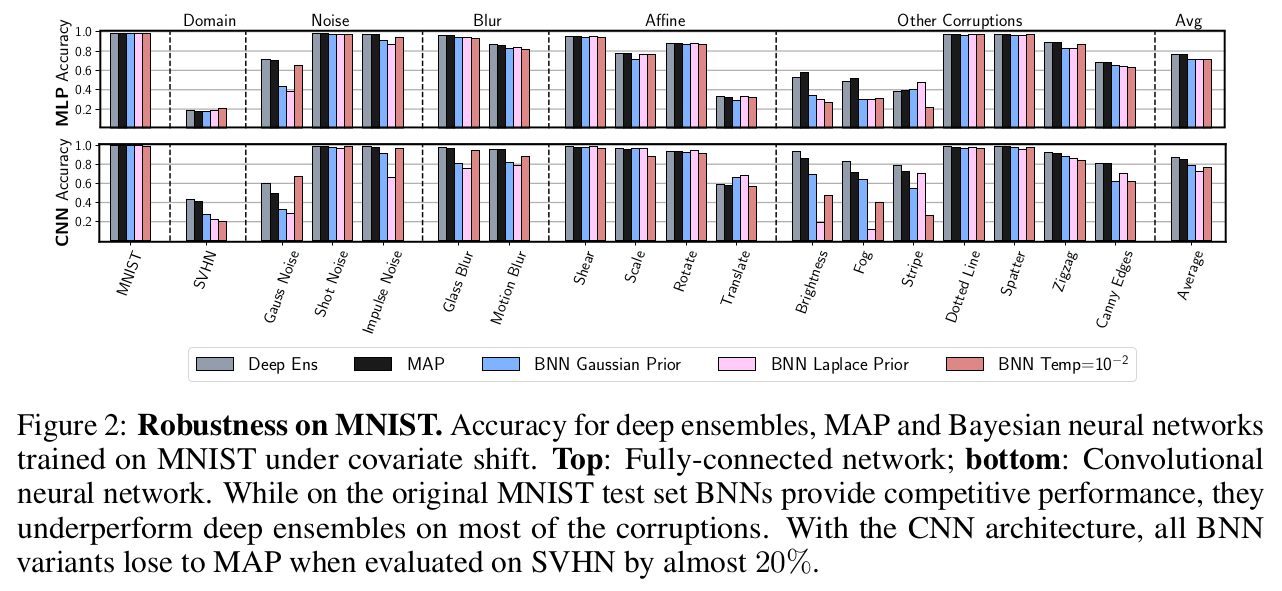
\includegraphics[scale=0.26]{figure2.png}
\end{frame}

\begin{frame}{}
\begin{block}{Domain shift}
    Next, we apply our CIFAR-10 CNN model to the STL-10 dataset. Both datasets contain natural
    images with 9 shared classes between the two datasets. We report the accuracy of the CIFAR-10
    models on these 9 shared classes in STL-10.
\end{block}
    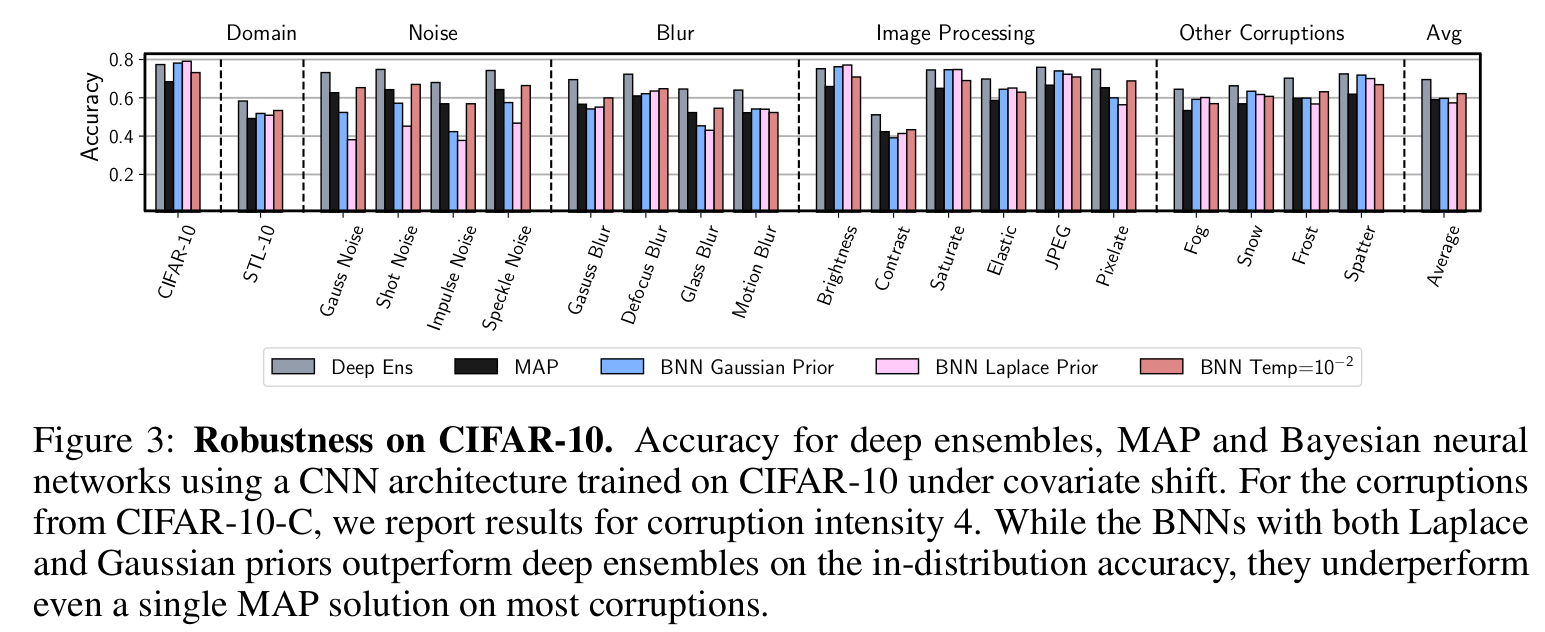
\includegraphics[scale=0.22]{figure3.png}
\end{frame}

\section{Explanation}
\begin{frame}{}
    \begin{block}{Understanding BNNs under covariate shift}
        We identify the linear dependencies in the input features as one of the key issues undermining the robustness of BNNs.

    \end{block}
    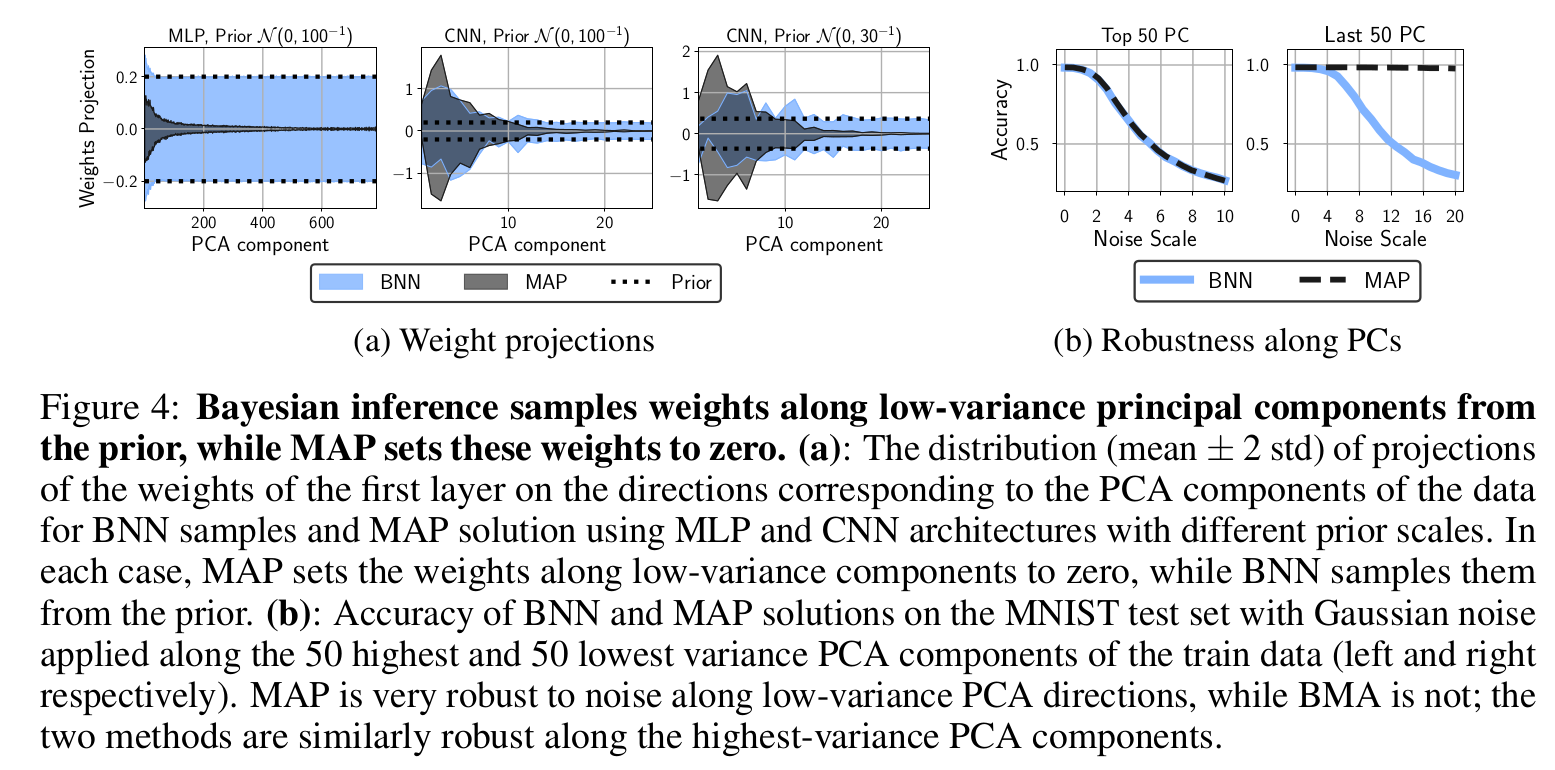
\includegraphics[scale=0.22]{figure4.png}
\end{frame}


\begin{frame}{}
    \begin{block}{Data empirical covariance prior}
        Assuming the input features are all preprocessed to be zero-mean, we have 
        $\Sigma = \frac 1 {n-1} \sum x_i x_i^T$. For fully-connected
        networks, we propose to use the $EmpCov$ prior $p(w ) = N (0, \alpha \Sigma + \varepsilon I)$ on the weights $w^1$ of the
        first layer of the network. The hyperparameter $\alpha > 0$ determines the scale of the prior.
    \end{block}
    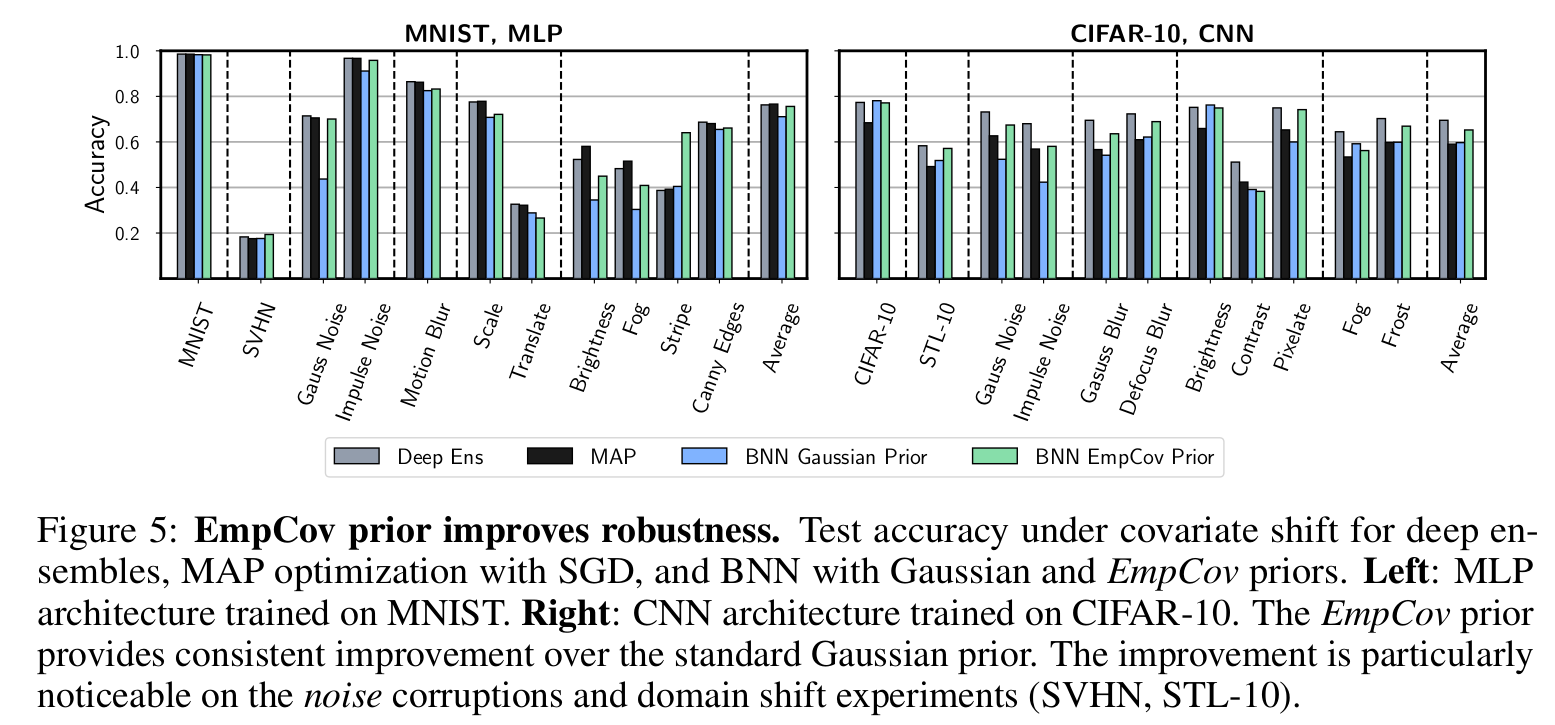
\includegraphics[scale=0.22]{figure5.png}
\end{frame}


\begin{frame}{Literature}
    \begin{enumerate}
        \item \textbf{Main article} \href{https://arxiv.org/pdf/2106.11905.pdf}
        {Dangers of Bayesian Model Averaging under Covariate Shift}
    \end{enumerate}
\end{frame}



\end{document}